To obtain a view on how the amount of crashes in the first section is influenced by various factors, Monte Carlo simulations are being used. Each simulation represents a start of a Grand Prix, in which every car attempts to pass the first turn. These cars, with an average length of five metres, and a width of two, start at a grid with two sides. Every other car starts left, or right, based on the first (pole) position (predefined for every circuit), with 8 metres in between \cite{car-regulations}, on a so called grid. For our simulation we divided the total width of the circuit in five lanes, to make it possible to overtake cars on both sides, as seen from both start rows.

There are 20 cars in each race. And in the simulations, every track of the 2017 Formula 1 calendar is being tested, 20 in total. The order in which the cars start, is sampled in each simulation out of all achieved qualification results in this season so far (16). By doing this, the possibilty that a driver had a bad day, or penalty can be neglected. When the driver within a team is switched during the season, this will be taken in advance.

To mimic the real world, behaviour of drivers/cars is based on the four steps used in the Nagel-Schreckenberg model:\\

\noindent
(1) acceleration\\
(2) slowing down\\
(3) randomization\\
(4) car motion

\smallskip
As long as the point of where a car should brake isn't reached, the car accelerates (1). The numbers being used to calculate the amount of metres that is added every second, are based on a few cars \cite{som}, and define the range for all cars.

When the 'braking zone' is (nearly) reached, the negative acceleration (2) is being calculated. The number is based on the current speed of the car together with the maximum speed that can be driven in the turn. This speed diminution will be devided over the amount of metres that's left for the turn.\cite{som}.

\begin{figure}[H]
\includegraphics[width=7cm]{f1start-01}
\caption{Model used for representation of circuits}
\end{figure}

Next to improving the distance driven, the driver will attempt to move to an optimal position on the track (4). What's optimal for a car at a certain moment differs. Ideally, if a car is faster than the car in front, it will try to overtake. Overtakes will be done with the 'optimal row' \footnote{The opposite side of the turn is considered as being optimal. By driving there, you could maintain the top speed/accelerate as long as possible.} in consideration.

When a car is in front of another car which is considered faster, it will try to defend its position by moving towards the row the car in the back is driving, in order to 'block' it.

Driving into the braking zone also means that an optimal position should be chosen to drive into the turn.

Sometimes when a car is faster, has the plan to defend or to improve its position, other cars are blocking this, or the car needs to go off the track to obtain the result. In this case the current position on track will be maintained.

\subsection{Crashes}
Checks for crash occurences will be executed till the second in which the car has passed the point of the first turn.

A check validates if something happend between the current car, and the car in front of it. By doing this, it's possible to check if the manouvre which just was executed, either accelerating, braking or switching could be performed succesfully.

Crashes can only happen between cars that are in the same row. If a crash is near, an additional switch of rows may be performed to avoid a crash. When no positive options are left, the driver has the option to brake, or crash. A choice out of these two will be made randomly (3). If the distance between the current car and the car in front is less than zero, this will be considered as a crash.

\begin{figure}[H]
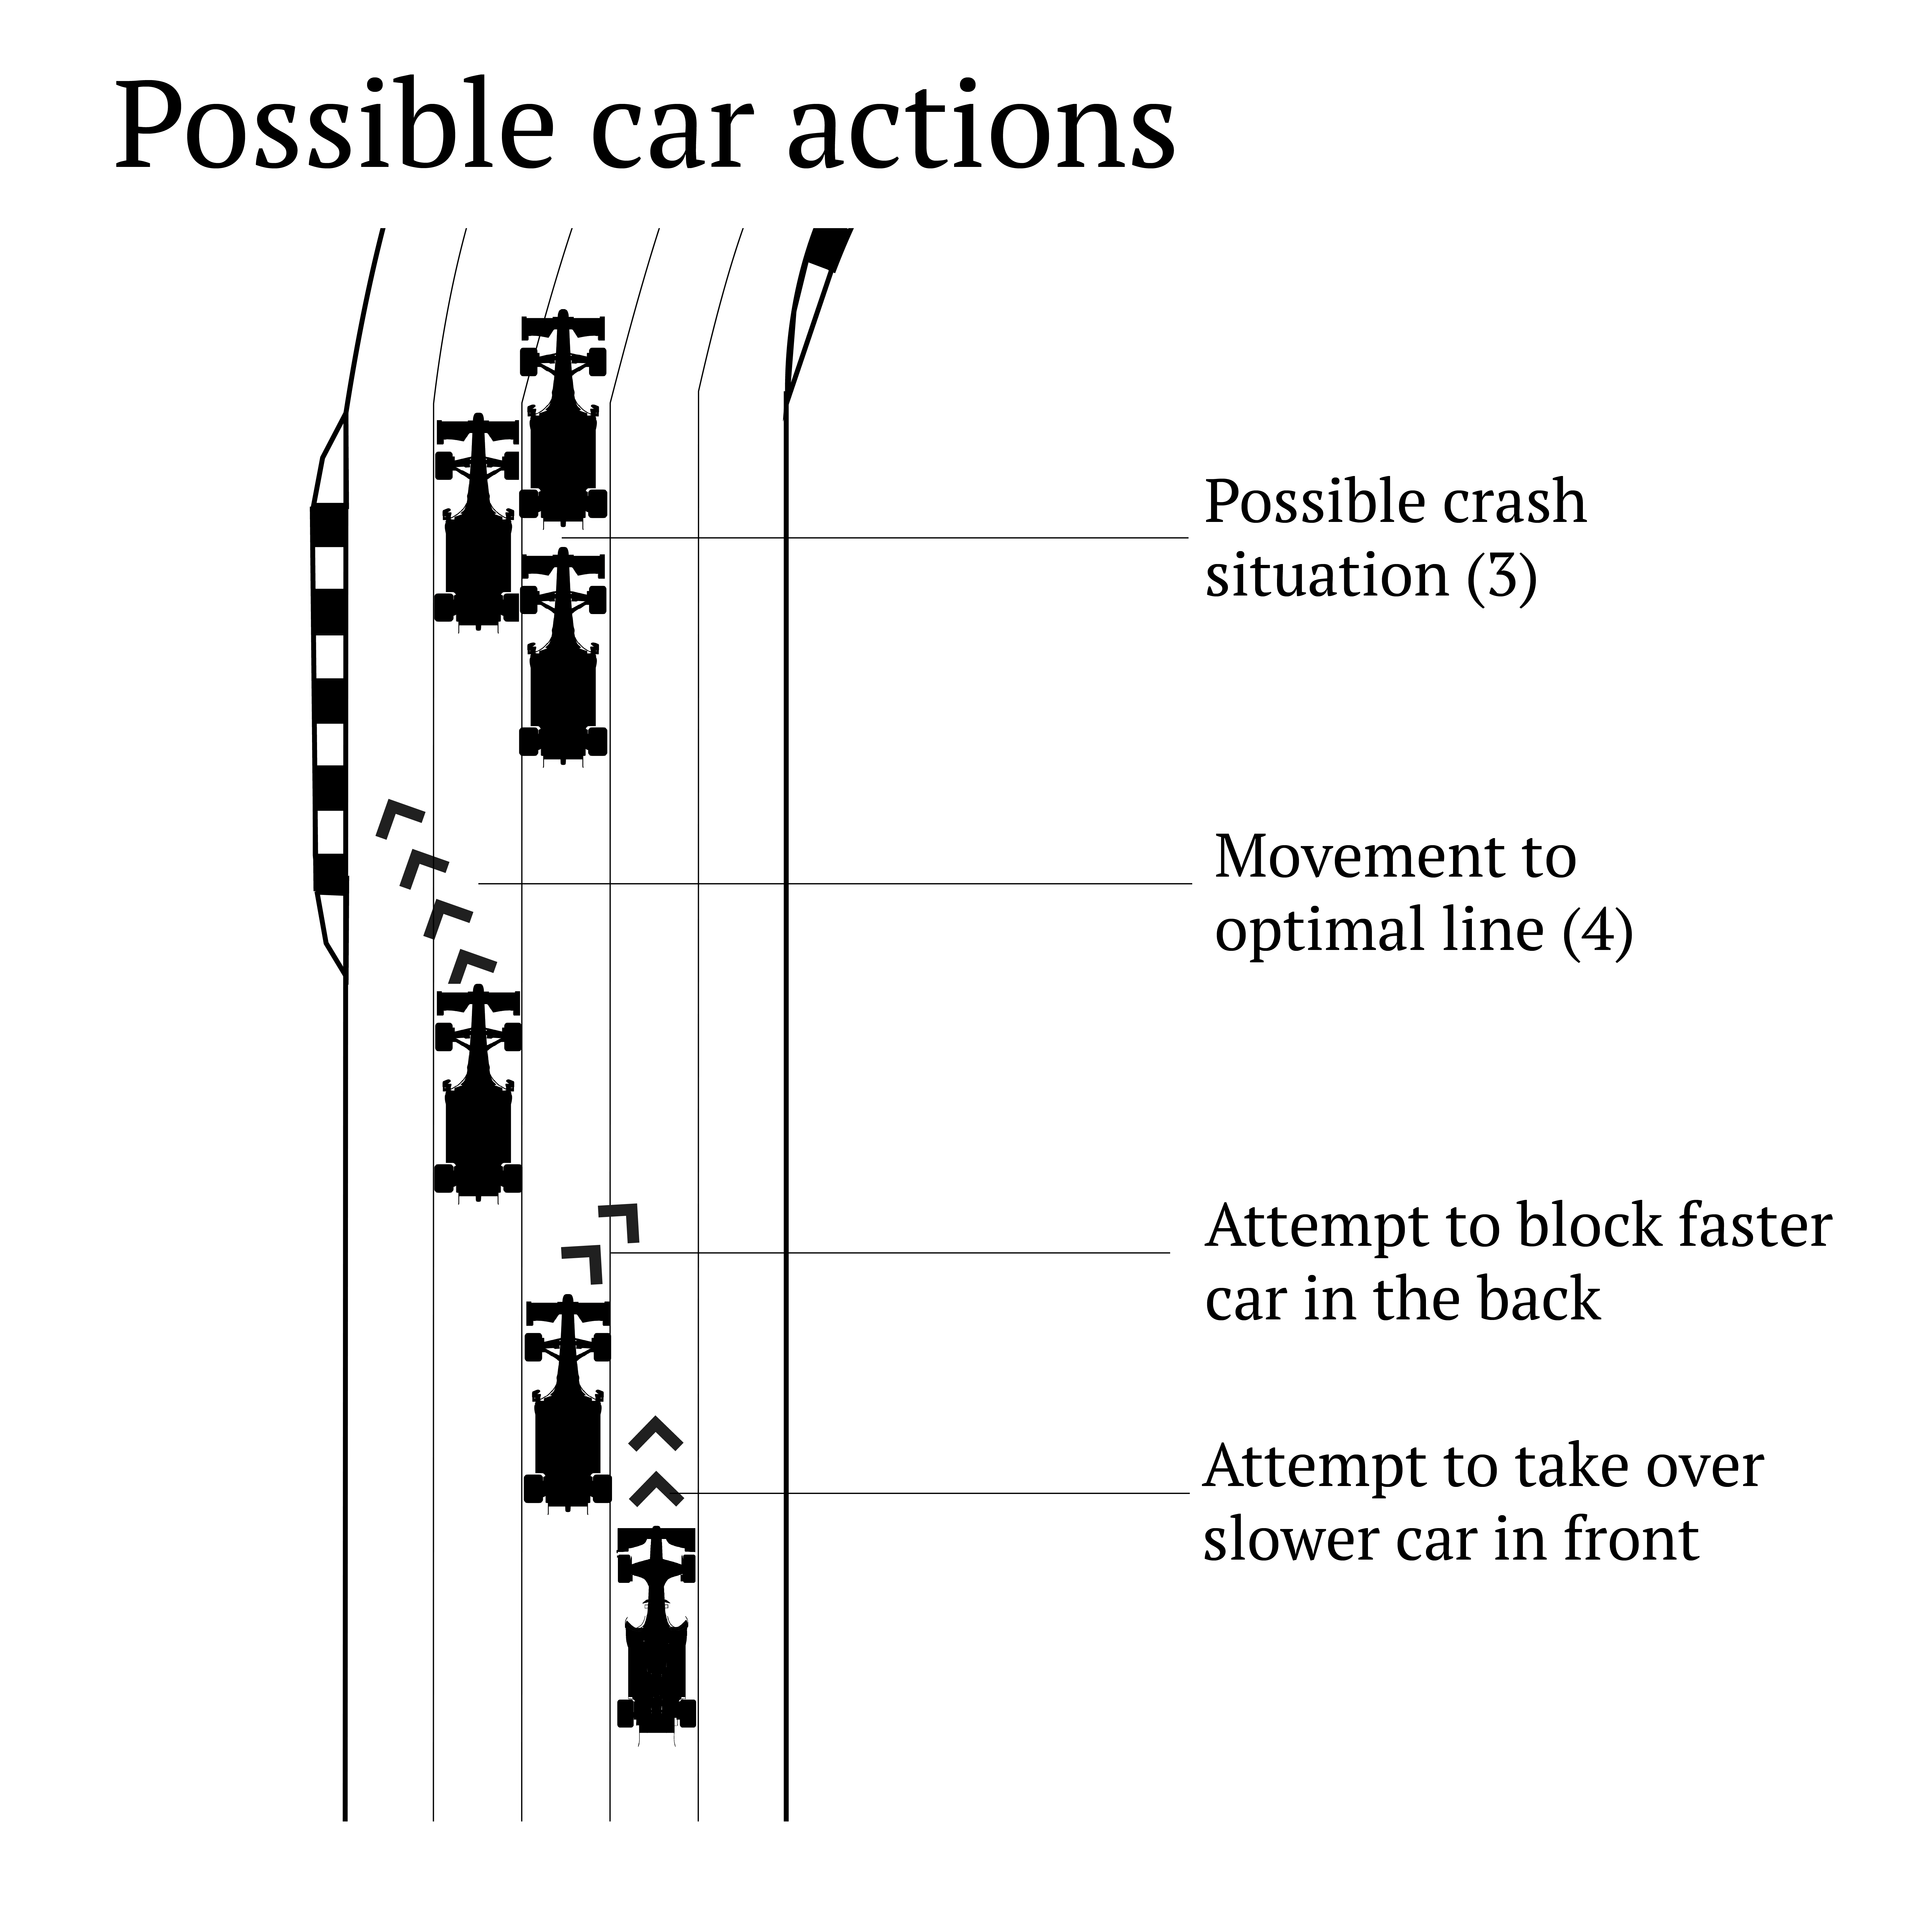
\includegraphics[width=7cm]{f1start-02}
\caption{Model used for car actions}
\end{figure}
